\documentclass[11pt]{article}
\usepackage[margin=1in,letterpaper]{geometry}
\usepackage{amsmath,amssymb}
\usepackage{graphicx}
\usepackage{booktabs}
\usepackage{tikz}
\usepackage[hidelinks]{hyperref}
\usepackage{caption}
\captionsetup{font=small,labelfont=bf}
\usetikzlibrary{arrows.meta,calc,decorations.pathmorphing,patterns}
\newcommand{\Aheld}{98}
\newcommand{\An}{100}
\newcommand{\Apiv}{73}
\newcommand{\AlsRms}{0.009}
\newcommand{\AlsMed}{0.005}
\newcommand{\AlsPnf}{0.016}
\newcommand{\AlsHor}{0.015}
\newcommand{\AlsTilt}{0.006}
\newcommand{\AnHor}{26}
\newcommand{\AlsRod}{0.066}
\newcommand{\AnaiveRod}{0.086}
\newcommand{\Agap}{0.065}
\newcommand{\AgapPnf}{0.129}
\newcommand{\ArOverDhi}{1.53}
\newcommand{\AampLo}{0.0093}
\newcommand{\AampHi}{0.0094}
\newcommand{\Bnd}{36}
\newcommand{\Bnu}{44}
\newcommand{\BratLo}{0.87}
\newcommand{\BratHi}{1.12}
\newcommand{\BuMed}{6.5}
\newcommand{\BuHi}{26.7}
\newcommand{\Bconfigs}{80}
\newcommand{\BsweepLo}{0.0093}
\newcommand{\BsweepHi}{0.0094}
\newcommand{\BnaiveZero}{0.088}
\newcommand{\BnaiveMax}{1.39}
\newcommand{\BeightZero}{0.259}
\newcommand{\BeightFive}{0.021}
\newcommand{\BditherGain}{12}
\newcommand{\BchainTwelve}{0.0016}
\newcommand{\COnRms}{0.413}
\newcommand{\COnMed}{0.325}
\newcommand{\COnPnf}{0.687}
\newcommand{\COnFive}{2.5}
\newcommand{\COnTen}{2.5}
\newcommand{\COnRod}{0.411}
\newcommand{\COnDrop}{0}
\newcommand{\COoRms}{0.107}
\newcommand{\COoMed}{0.073}
\newcommand{\COoPnf}{0.197}
\newcommand{\COoFive}{30.0}
\newcommand{\COoTen}{72.5}
\newcommand{\COoRod}{0.060}
\newcommand{\COoDrop}{0}
\newcommand{\CCoRms}{0.027}
\newcommand{\CCoMed}{0.011}
\newcommand{\CCoPnf}{0.052}
\newcommand{\CCoFive}{92.5}
\newcommand{\CCoTen}{100.0}
\newcommand{\CCoRod}{0.053}
\newcommand{\CCoDrop}{0}
\newcommand{\CCoProbes}{16.4}
\newcommand{\CCoProbesMax}{23}
\newcommand{\CCoTsim}{2.4}
\newcommand{\CCcRms}{0.031}
\newcommand{\CCcMed}{0.013}
\newcommand{\CCcPnf}{0.068}
\newcommand{\CCcFive}{90.0}
\newcommand{\CCcTen}{97.5}
\newcommand{\CCcRod}{0.052}
\newcommand{\CCcDrop}{0}
\newcommand{\CCcProbes}{16.6}
\newcommand{\CCcProbesMax}{22}
\newcommand{\CCcTsim}{5.4}
\newcommand{\CccSelf}{0.008}
\newcommand{\Cn}{40}

\graphicspath{{../figures/}}
\newcommand{\sgn}{\operatorname{sgn}}

\title{Gravity Pivoting from Motor Current:\\ Calibration-Free Angle Estimation and the Sensing Budget It Requires}
\author{Clement Aidoo\\ CANLABS, Ghana\\ \texttt{aidooclement613@gmail.com}}
\date{October 2026 \quad (simulation study, preprint draft)}

\begin{document}
\maketitle

\begin{abstract}
Gravitational pivoting lets a parallel-jaw gripper reorient a grasped object by loosening its grip so that gravity rotates the object about the grasp axis. Published pivoting controllers observe the object with tactile sensors or cameras. We ask whether the motor current of the gripper's wrist actuator is enough. Under quasi-static conditions the wrist carries the gravity torque $mgr\cos(\theta+\psi)$, so a slow downhill sweep of the wrist angle $\psi$ while the object is clamped, followed by a linear least-squares fit, recovers the direction $\theta$ of the object's centre of mass. The estimate needs no object mass, grasp offset or motor torque constant, and a sign-of-velocity regressor removes gearbox Coulomb friction. In MuJoCo simulation with a soft-finger contact model and \An{} randomized objects, the estimator located the centre-of-mass direction to \AlsRms{}\,rad RMS with ideal sensing. Through a modelled current-sensing chain it stayed at \BsweepLo{}--\BsweepHi{}\,rad for gearbox friction up to 0.1\,N\,m, while a single static current reading degraded from \BnaiveZero{} to \BnaiveMax{}\,rad. A linearized error budget in ADC resolution and current noise matched simulation to within a factor of \BratLo{}--\BratHi{} whenever the noise exceeded half a quantization step, and failed by up to \BuHi{}$\times$ otherwise; adding noise improved an 8-bit sensor \BditherGain{}-fold. In closed loop, a controller using only motor current pivoted \Cn{} randomized objects to target angles with \CCcRms{}\,rad RMS error (\CCcFive\% within 0.05\,rad), against \COoRms{}\,rad for an open-loop schedule given the true object parameters and \COnRms{}\,rad for one given nominal parameters. We also report the limits we found: torque observes the centre-of-mass direction rather than the object's geometric axis, a wrist motion made while the grip is loose ratchets the object downward, and the controller needs about \CCcProbes{} probes per pivot. All results are from simulation.
\end{abstract}

\section{Introduction}
Pivoting is one of the simplest forms of in-hand manipulation. A parallel-jaw gripper holds a long object away from its centre of mass, reduces its grip force, and lets gravity rotate the object about the axis through the two contacts until friction stops it \cite{holladay2015,vina2016,toskov2023}. No extra fingers are needed, which makes pivoting attractive for the low-cost grippers that dominate outside research labs. Its difficulty is that the outcome depends on friction, which is poorly known, so closed-loop pivoting has relied on sensing the object directly: tactile arrays and vision in \cite{vina2016}, and tactile sensing with learned control in \cite{toskov2023}.

Tactile skins and cameras add cost, wiring and fragility. Every motorized joint, however, already measures one signal that carries load information: its motor current. Using actuator signals as a stand-in for touch has a long history in collision detection \cite{deluca2005}, and has recently been applied to compliant dexterous grasping \cite{ma2026}, damage-safe grasping \cite{shuto2026} and contact detection on low-cost arms \cite{zhu2026}. These works use current to detect or regulate contact. Here the question is whether current can measure the \emph{state} of a manipulated object, specifically its angle during gravity pivoting, and what electrical sensing quality that requires.

Three physical facts make the problem tractable and also set its limits. First, once an object is clamped, the wrist joint must carry the object's gravity torque, which depends on the direction of the object's centre of mass (COM) relative to the wrist axis. Second, a single torque reading confounds that direction with the COM distance, which changes when the object slides along its length in the grasp. Third, a geared motor's current also contains gearbox friction, which for small gearmotors can be as large as the gravity signal itself.

\paragraph{Contributions.}
\begin{enumerate}
\item A calibration-free estimator that recovers the COM direction from wrist motor current using a slow, one-sided wrist sweep and linear least squares. The motor torque constant, gear ratio, object mass and grasp offset all cancel, and Coulomb friction is removed by a regressor rather than identified separately (Section~\ref{sec:method}).
\item Two design rules for the probing motion, derived and checked in simulation: the sweep must move downhill so the clamped object stays inside its friction cone, and it must be slow because inertial torque is affine in the wrist angle for a single-frequency sweep and cannot be separated from gravity by the fit.
\item A sensing budget: a closed-form, linearized prediction of angle error from ADC resolution and current noise, validated against \Bconfigs{} simulated sensing chains, with the regime where it fails (undithered quantization) identified (Section~\ref{sec:expB}).
\item A closed-loop pivoting controller that uses only motor current and reaches target angles more accurately than an open-loop schedule given the true object parameters (Section~\ref{sec:expC}).
\end{enumerate}
We report negative results alongside these: what torque cannot observe, a wrist-dither controller that failed, and the cost in probing time.

\section{Related Work}
\paragraph{Pivoting.} Holladay et al.\ \cite{holladay2015} plan open-loop pivoting trajectories using a friction model of the grasp. Vi\~na et al.\ \cite{vina2016} close the loop with vision and tactile feedback and adapt to unknown friction. Toskov et al.\ \cite{toskov2023} learn gravitational pivoting with tactile sensing. Our controller targets the same task without any sensor beyond the actuators.

\paragraph{Soft-finger contact.} The torsional friction that resists pivoting is captured by the soft-finger contact model, in which each contact can transmit a torque about its normal bounded by a torsional coefficient times the normal force \cite{xydas1999}. We use this model both in simulation and in the controller.

\paragraph{Actuator signals as contact sensors.} Momentum-observer methods detect collisions from motor torques without force sensors \cite{deluca2005}. Recent work learns compliance references from motor current and joint states on dexterous hands \cite{ma2026}, classifies grasps as safe, slipping or damaging from servo effort \cite{shuto2026}, and improves proprioceptive contact detection on low-cost arms by predicting contact-free torques \cite{zhu2026}. These use current to detect or regulate contact. We use it to estimate a continuous object state and quantify the sensing chain needed to do so.

\paragraph{Friction and quantization.} Coulomb and viscous friction terms in actuator models are standard \cite{armstrong1994}. That a quantizer's error behaves like additive uniform noise only when the input is sufficiently dithered is classical \cite{gray1993}; we find the same boundary governs whether our error budget holds.

\section{Model}\label{sec:model}
\begin{figure}[t]
\centering
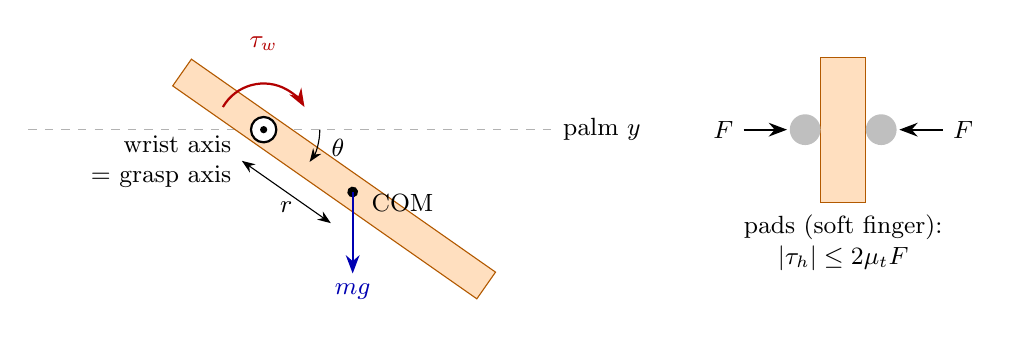
\begin{tikzpicture}[scale=1.15,>=Stealth]
  % palm frame
  \draw[gray!60,dashed] (-2.6,0) -- (3.2,0) node[right,black,font=\small]{palm $y$};
  % rod rotated by theta
  \begin{scope}[rotate=-35]
    \fill[orange!25,draw=orange!70!black] (-1.1,-0.18) rectangle (3.0,0.18);
    \fill[black] (1.2,0) circle (0.06);
    \draw[<->,thin] (0,-0.42) -- node[below,font=\small]{$r$} (1.2,-0.42);
  \end{scope}
  % wrist axis
  \draw[thick,fill=white] (0,0) circle (0.14); \fill (0,0) circle (0.04);
  \node[font=\small,anchor=east,align=right] at (-0.25,-0.35) {wrist axis\\$=$ grasp axis};
  % angle
  \draw[->] (0.62,0) arc (0:-35:0.62); \node[font=\small] at (0.82,-0.2) {$\theta$};
  % gravity at COM
  \coordinate (C) at ({1.2*cos(-35)},{1.2*sin(-35)});
  \node[font=\small,right] at ($(C)+(0.1,-0.12)$) {COM};
  \draw[->,thick,blue!70!black] (C) -- ++(0,-0.9) node[below,font=\small]{$mg$};
  % wrist torque
  \draw[->,thick,red!70!black] (-0.45,0.25) arc (150:30:0.52); \node[red!70!black,font=\small] at (0,0.95) {$\tau_w$};
  % inset: pads
  \begin{scope}[shift={(6.4,0)}]
    \fill[orange!25,draw=orange!70!black] (-0.25,-0.8) rectangle (0.25,0.8);
    \fill[gray!50] (-0.42,0) circle (0.17); \fill[gray!50] (0.42,0) circle (0.17);
    \draw[->,thick] (-1.1,0) -- (-0.62,0) node[pos=0,left,font=\small]{$F$};
    \draw[->,thick] (1.1,0) -- (0.62,0) node[pos=0,right,font=\small]{$F$};
    \node[font=\small,align=center] at (0,-1.25) {pads (soft finger):\\ $|\tau_h| \le 2\mu_t F$};
  \end{scope}
\end{tikzpicture}
\caption{Gravity pivoting about the grasp axis. Left: view along the grasp axis, which coincides with the wrist axis. The COM lies at distance $r$ and direction $\theta$ in the palm frame. Right: the two pads squeeze the object with force $F$ each; the soft-finger torsional friction bounds the holding torque about the grasp axis.}
\label{fig:setup}
\end{figure}

\paragraph{Pivot equilibrium.} Let the object (mass $m$) be held so that its COM lies a distance $r$ from the grasp axis, at angle $\theta$ below the palm's horizontal (Fig.~\ref{fig:setup}), with the wrist at angle $\psi$. The gravity torque about the grasp axis is $mgr\cos(\theta+\psi)$. With soft-finger contacts of torsional coefficient $\mu_t$ \cite{xydas1999}, the two pads can resist at most $2\mu_t F$, so with the wrist fixed at $\psi=0$ a quasi-static pivot comes to rest where
\begin{equation}
\cos\theta^\star = \frac{2\mu_t F}{mgr}. \label{eq:equilibrium}
\end{equation}
An open-loop pivoting schedule inverts \eqref{eq:equilibrium} for $F$, which requires $m$, $r$ and $\mu_t$.

\paragraph{Wrist statics and actuator.} While the object is stuck to the pads, the wrist must supply $\tau_w = mgr\cos(\theta+\psi)$. A brushed DC gearmotor with torque constant $K_t$, gear ratio $N$, output-referred Coulomb friction $\tau_c$, viscous coefficient $b$ and reflected rotor inertia $J_r$ draws current
\begin{equation}
N K_t\, i = mgr\cos(\theta+\psi) + \tau_c \sgn\dot\psi + b\dot\psi + J_r\ddot\psi + J_o\ddot\psi, \label{eq:motor}
\end{equation}
where $J_o$ is the unmodelled inertia of the palm and object. The current is measured by a $B$-bit converter with full scale $\pm I_{fs}$ and quantization step $\Delta = 2I_{fs}/2^B$, after additive noise of standard deviation $\sigma_n$. At rest, $\sgn\dot\psi$ is undefined and stiction can take any value in $[-\tau_c,\tau_c]$.

\paragraph{What one reading can and cannot tell.} A single reading at rest gives $mgr\cos\theta$ plus an unknown stiction term. Even with stiction absent and a calibration reading $mgr_0$ taken at $\theta=0$, the estimate $\arccos(\tau_w/mgr_0)$ assumes $r=r_0$. In our simulations the COM distance changed during pivoting by up to a factor of \ArOverDhi{} because the object also slid along its length, so a single reading cannot separate angle from slide.

\section{Method}\label{sec:method}
\subsection{Sweep estimator}
With the object clamped (large $F$), the wrist executes a one-sided sweep $\psi(t) = -\delta\,(1-\cos\omega t)$ over one period. Substituting $\cos(\theta+\psi) = \cos\theta\cos\psi - \sin\theta\sin\psi$ into \eqref{eq:motor} gives a model linear in its unknowns,
\begin{equation}
i(t) = a\cos\psi + b\sin\psi + c\,\sgn\dot\psi + v\,\dot\psi + e(t), \qquad a = \tfrac{mgr\cos\theta}{NK_t},\; b = -\tfrac{mgr\sin\theta}{NK_t}, \label{eq:regression}
\end{equation}
after subtracting the datasheet rotor-inertia term $J_r\ddot\psi_{\mathrm{cmd}}/(NK_t)$. Ordinary least squares gives $(a,b,c,v)$ and
\begin{equation}
\hat\theta = \operatorname{atan2}(-b,\,a).
\end{equation}
Because $\hat\theta$ depends only on the ratio $b/a$, the factor $mgr/(NK_t)$ cancels: the estimator needs neither the object's mass and grasp offset nor the motor's torque constant and gear ratio. On the outbound and return halves of the sweep the wrist visits the same angles with opposite $\sgn\dot\psi$, which makes the Coulomb term identifiable from the same data.

\subsection{Two design rules for the probe}
\paragraph{Downhill only.} The probe must not itself make the object slip. Rotating the wrist so that the COM moves toward the horizontal raises the gravity torque on the contacts, and in early tests this made the object slip even under a firm clamp. Sweeping only toward the vertical lowers the gravity torque for objects that hang no further than vertical, so the clamped object stays inside its friction cone; this is why the sweep is one-sided.

\paragraph{Slow, because inertia is invisible to the fit.} For the single-frequency sweep above, $\ddot\psi = \omega^2(\psi+\delta)$ is affine in $\psi$. Any unmodelled inertia $J_o$ therefore adds a term that the regressors $\cos\psi\approx 1$ and $\sin\psi\approx\psi$ absorb into $a$ and $b$, biasing $\hat\theta$ by roughly $J_o\omega^2/(mgr)$ in the $\sin\theta$ direction. In simulation, raising the sweep frequency from 0.1 to 0.2\,Hz increased the error three- to fourfold on several test objects, and a 1\,Hz rolling estimate during a grip release (Section~\ref{sec:expC}) was unusable. We use 0.1\,Hz and $\delta=0.15$\,rad (a 0.3\,rad range).

\subsection{Error budget}
Treating quantization as uniform noise of variance $\Delta^2/12$ added to $\sigma_n^2$, the covariance of the coefficients is $\Sigma = (\sigma_n^2 + \Delta^2/12)(X^\top X)^{-1}$, with $X$ the regressor matrix of \eqref{eq:regression}. Linearizing $\hat\theta$ gives
\begin{equation}
\operatorname{Var}\hat\theta \approx g^\top \Sigma\, g, \qquad g = \frac{1}{a^2+b^2}\,[\,b,\; -a,\; 0,\; 0\,]^\top. \label{eq:budget}
\end{equation}
The leading behaviour is $\sigma_\theta \propto \sqrt{\sigma_n^2+\Delta^2/12}\,/\,(A\,\delta\sqrt{n})$, with $A=\sqrt{a^2+b^2}$ and $n$ samples, so accuracy degrades for light objects, small offsets and small sweeps. The uniform-noise assumption holds only when the input is dithered \cite{gray1993}; Section~\ref{sec:expB} tests where \eqref{eq:budget} breaks.

\subsection{Closed-loop pivoting controller}\label{sec:controller}
Gravity can only rotate the object further down, so overshoot cannot be undone. The controller therefore approaches the target from above in measured steps:
\begin{enumerate}
\item Clamp and probe to obtain $\hat\theta_0$ and $\hat A$. Convert $\hat A$ to a gravity torque with the nominal motor constant (a $\pm10\%$ error is injected) and set the first release force from a conservative lower bound on $\mu_t$.
\item Release the grip slowly (0.3\,N/s) to the planned force, re-clamp with a 0.5\,s force ramp, and probe.
\item Until the estimate has moved by 0.03\,rad, reduce the planned force by 6\% per step. Afterwards, fit $c = \cos\hat\theta/F$ at the last equilibrium, as in \eqref{eq:equilibrium}, and plan the next force to cover 70\% of the remaining angle.
\item Stop when $\hat\theta$ is within 0.03\,rad of the target or past it.
\end{enumerate}
Each release first ramps quickly to 1.05 times the previous release force, where the object is known to hold, and only then slowly. The wrist does not move while the grip is low.

\section{Experimental Setup}
\paragraph{Simulator.} We use MuJoCo 3.15 \cite{todorov2012} at a 1\,ms step with the implicit-fast integrator, elliptic friction cones and 20 no-slip iterations. Each pad is a 6\,mm sphere on a prismatic joint driven by a force actuator, and pad--object contacts use \texttt{condim=4} (sliding plus torsional friction). The object is a $2\times16\times2$\,cm box on a free joint; the wrist is a hinge driven by a position servo whose actuator force is the simulated output torque $\tau_w$. This testbed replaces an earlier PyBullet model in which torsional resistance arose only from the spread of box--box contact points; there, a clamped object crept by up to 0.37\,rad, which is unacceptable for a study about torsional holding. A preliminary version of this work also contained an evaluation error, documented separately \cite{aidoo2026}.

\paragraph{Validation of the physics.} With a slow grip release (0.2\,N/s) the object tracked the equilibrium \eqref{eq:equilibrium} to within 0.11\,rad, and the pivot began between 4.8 and 5.2\,N against a predicted threshold of 4.9\,N. Two simulator artifacts surfaced and were handled: an instantaneous change of grip force excited a sustained normal-force oscillation between the pads (removed by ramping the clamp over 0.5\,s), and soft torsional contacts produced a velocity-proportional lag of about 0.01\,rad between the object and the palm during probing (absorbed by the $\dot\psi$ regressor). We checked that no Exp~A probe showed slip beyond this lag.

\paragraph{Randomization.} Objects draw $m\in[0.05,0.2]$\,kg, grasp offset $d\in[2,6]$\,cm, $\mu\in[0.4,0.8]$ and $\mu_t\in[2,6]$\,mm. In Exp~A the release force is $F^\ast\cdot U(0.3,1.3)$, with $F^\ast = mgd/(2\mu_t)$ the pivot threshold. Exp~C targets draw $\theta^\star\in[-1.3,-0.3]$\,rad.

\paragraph{Sensing chain.} The actuator model \eqref{eq:motor} uses $N=100$, $K_t = 0.0107$\,N\,m/A, $J_r = 2\times10^{-7}\cdot N^2$\,kg\,m$^2$, $b = 0.002$\,N\,m\,s/rad and $I_{fs}=2$\,A, values representative of a small 12\,V brushed gearmotor rather than any particular part. Because the sensing chain does not feed back into the physics during an open-loop probe, Exp~B applies it to recorded torque traces, which lets one simulation serve many sensing configurations.

\section{Results}
\subsection{Exp A: estimator accuracy with ideal sensing}
Of \An{} randomized trials, \Aheld{} kept the object and \Apiv{} pivoted by more than 0.1\,rad. Table~\ref{tab:expA} summarizes the errors.
\begin{table}[h]
\centering\small
\begin{tabular}{lc}
\toprule
Quantity & RMS error (rad) \\
\midrule
Sweep estimate vs.\ COM direction (all held) & \AlsRms{} \\
\quad near horizontal, $|\sin\theta|<0.3$ ($n=\AnHor{}$) & \AlsHor{} \\
\quad tilted, $|\sin\theta|\ge 0.3$ & \AlsTilt{} \\
Sweep estimate vs.\ object's geometric angle & \AlsRod{} \\
Single static reading vs.\ object's geometric angle & \AnaiveRod{} \\
COM direction vs.\ geometric angle (in-grasp translation) & \Agap{} \\
\bottomrule
\end{tabular}
\caption{Exp A: ideal sensing, sweep amplitude 0.15\,rad, \Aheld{} held trials. For the first row the median error was \AlsMed{}\,rad and the 95th percentile \AlsPnf{}\,rad; the 95th percentile of the COM--geometric gap was \AgapPnf{}\,rad.}
\label{tab:expA}
\end{table}

The sweep recovers the COM direction to \AlsRms{}\,rad RMS. Accuracy is worse near the horizontal, where $\partial\tau_w/\partial\theta \propto \sin\theta$ is small, as \eqref{eq:budget} predicts. Measured against the object's geometric axis, the error rises to \AlsRod{}\,rad, which is close to the \Agap{}\,rad gap between COM direction and geometric axis. That gap comes from the object translating sideways in the grasp, which no wrist-torque measurement can observe. On this geometric-angle measure the sweep improves on a single static reading (\AnaiveRod{}\,rad) by about a quarter; the larger advantage appears once realistic friction is added (Exp~B). With ideal sensing, the RMS error was the same (\AampLo{}--\AampHi{}\,rad) for sweep amplitudes of 0.075, 0.15 and 0.3\,rad.

\subsection{Exp B: the sensing budget}\label{sec:expB}
We applied \Bconfigs{} sensing configurations (5 resolutions $\times$ 4 noise levels $\times$ 4 friction levels, four noise draws each) to the Exp~A traces.

\begin{figure}[t]
\centering
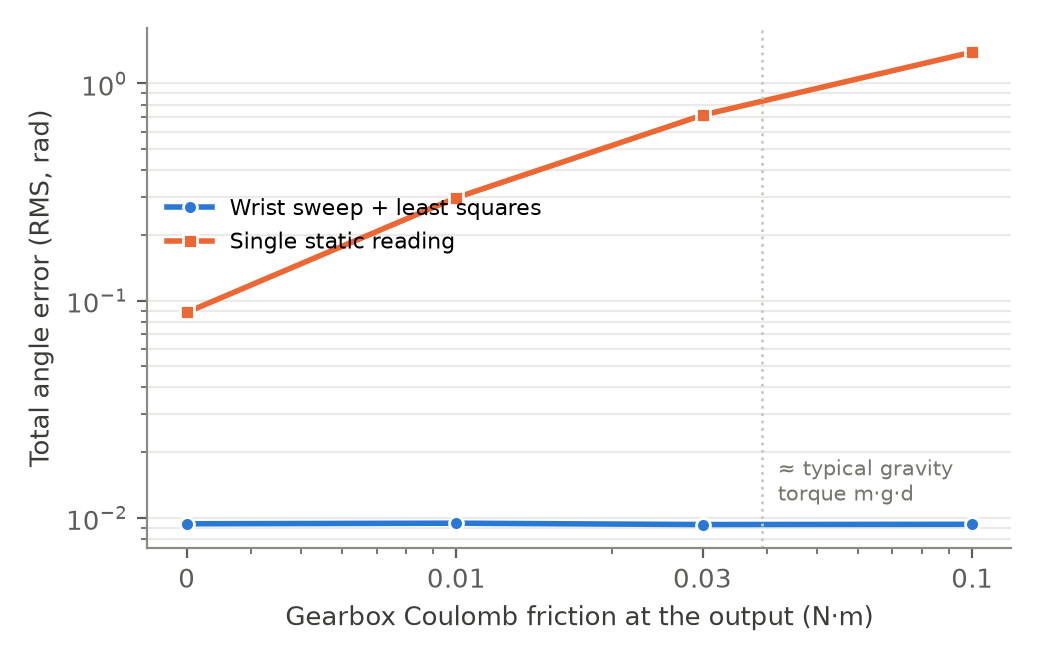
\includegraphics[width=0.62\linewidth]{fig_friction.png}\\[4pt]
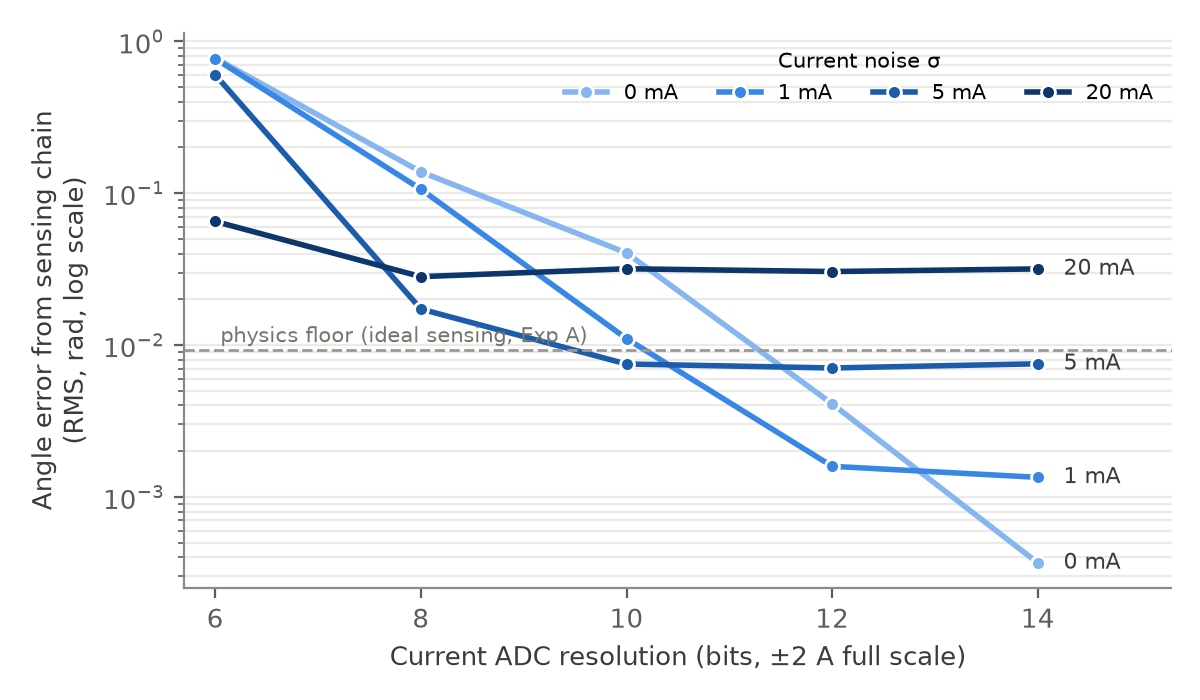
\includegraphics[width=0.72\linewidth]{fig_bits.png}
\caption{Top: total angle error against gearbox Coulomb friction (12-bit, 1\,mA noise). The zero-friction point is drawn at the left edge of the log axis. Bottom: error due to the sensing chain alone against ADC resolution for four current-noise levels ($\tau_c=0.03$\,N\,m); the dashed line is the ideal-sensing error of Exp~A.}
\label{fig:expB}
\end{figure}

\paragraph{Friction.} With a 12-bit converter and 1\,mA noise, the sweep's total error stayed between \BsweepLo{} and \BsweepHi{}\,rad as Coulomb friction rose from 0 to 0.1\,N\,m, about 2.3 times the median gravity torque $mgd$ in our object set (Fig.~\ref{fig:expB}, top; Table~\ref{tab:fric}). The single static reading, which cannot know the sign of stiction, degraded from \BnaiveZero{} to \BnaiveMax{}\,rad.

\paragraph{Resolution and noise.} Error from the sensing chain fell with resolution until it reached a floor set by current noise (Fig.~\ref{fig:expB}, bottom; Table~\ref{tab:bits}). Up to 12 bits, moderate noise helped: at 8 bits and zero friction, the error was \BeightZero{}\,rad without noise and \BeightFive{}\,rad with 5\,mA of noise, a \BditherGain{}-fold improvement, because noise dithers the quantizer and lets averaging over the sweep recover sub-LSB information. With about 1\,mA noise, 12 bits brought the sensing-chain error to \BchainTwelve{}\,rad, well below the \AlsRms{}\,rad set by the simulated physics.

\begin{table}[h]
\centering\small
\begin{minipage}{0.56\linewidth}\centering
\begin{tabular}{lccccc}
\toprule
$\sigma_n$ (mA) & 6 bit & 8 bit & 10 bit & 12 bit & 14 bit \\
\midrule
0 & 0.7740 & 0.1380 & 0.0404 & 0.0041 & 0.0004 \\
1 & 0.7683 & 0.1061 & 0.0110 & 0.0016 & 0.0013 \\
5 & 0.6008 & 0.0172 & 0.0075 & 0.0071 & 0.0075 \\
20 & 0.0651 & 0.0282 & 0.0318 & 0.0305 & 0.0317 \\

\bottomrule
\end{tabular}
\caption{Sensing-chain RMS error (rad), $\tau_c = 0.03$\,N\,m, $I_{fs}=\pm2$\,A.}
\label{tab:bits}
\end{minipage}\hfill
\begin{minipage}{0.4\linewidth}\centering
\begin{tabular}{ccc}
\toprule
$\tau_c$ (N\,m) & Sweep & Static \\
\midrule
0 & 0.0094 & 0.088 \\
0.01 & 0.0094 & 0.298 \\
0.03 & 0.0093 & 0.715 \\
0.1 & 0.0093 & 1.394 \\

\bottomrule
\end{tabular}
\caption{Total RMS error (rad), 12 bit, 1\,mA.}
\label{tab:fric}
\end{minipage}
\end{table}

\paragraph{When the budget holds.} Figure~\ref{fig:pred} compares the prediction \eqref{eq:budget} with the measured sensing-chain error. For the \Bnd{} configurations with $\sigma_n \ge \Delta/2$, measured error was \BratLo{}--\BratHi{} times the prediction. For the \Bnu{} configurations with less noise, the median ratio was \BuMed{} and the worst \BuHi{}: quantization error is then deterministic and correlated across samples, so the uniform-noise model and the $1/\sqrt{n}$ averaging it implies no longer apply \cite{gray1993}. For design purposes the rule is simple: size the converter so that $\Delta/2 \lesssim \sigma_n$, or add dither, and \eqref{eq:budget} then gives the expected accuracy.

\begin{figure}[t]
\centering
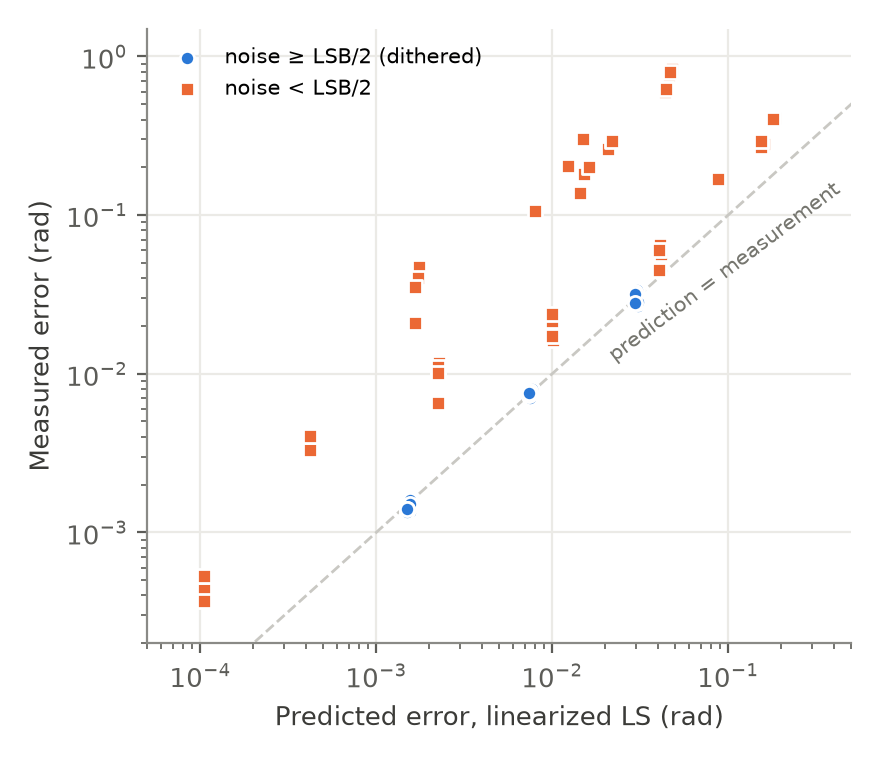
\includegraphics[width=0.48\linewidth]{fig_predicted.png}
\caption{Predicted (linearized least squares) against measured sensing-chain error for all \Bconfigs{} configurations. Circles: noise at least half a quantization step. Squares: less noise.}
\label{fig:pred}
\end{figure}

\subsection{Exp C: closed-loop pivoting from motor current}\label{sec:expC}
Each of \Cn{} randomized objects was pivoted to a random target with four methods, all starting from the same clamped horizontal grasp and releasing at the same slow rate. The closed-current controller used the full sensing chain (12 bit, 1\,mA, $\tau_c = 0.03$\,N\,m, $\pm10\%$ motor-constant error). The closed-oracle controller ran the same logic with the true angle in place of the estimate.

\begin{table}[h]
\centering\small
\begin{tabular}{lcccccc}
\toprule
Method & RMS & Median & 95th pct. & $\le$0.05\,rad & $\le$0.1\,rad & Geom.\ RMS \\
\midrule
Open loop, nominal object & \COnRms & \COnMed & \COnPnf & \COnFive\% & \COnTen\% & \COnRod \\
Open loop, true $m$, $d$, $\mu_t$ & \COoRms & \COoMed & \COoPnf & \COoFive\% & \COoTen\% & \COoRod \\
Closed loop, true angle & \CCoRms & \CCoMed & \CCoPnf & \CCoFive\% & \CCoTen\% & \CCoRod \\
Closed loop, motor current only & \CCcRms & \CCcMed & \CCcPnf & \CCcFive\% & \CCcTen\% & \CCcRod \\
\bottomrule
\end{tabular}
\caption{Exp C: final error to the target COM direction (rad) over \Cn{} objects. ``Geom.\ RMS'' scores the same runs against the object's geometric angle. No object was dropped by any method.}
\label{tab:expC}
\end{table}

Using motor current alone, the controller reached the target with \CCcRms{}\,rad RMS error (Table~\ref{tab:expC}, Fig.~\ref{fig:expC}), within 0.004\,rad of the same controller given the true angle, and its own final estimate was within \CccSelf{}\,rad RMS of the truth. Open-loop schedules failed even with perfect object knowledge: given the true $m$, $d$ and $\mu_t$, the open-loop release overshot on average and reached 0.05\,rad in only \COoFive\% of trials, consistent with the lag between the object and the equilibrium \eqref{eq:equilibrium} that we measured during continuous releases. With nominal parameters the open-loop error was \COnRms{}\,rad.

\begin{figure}[t]
\centering
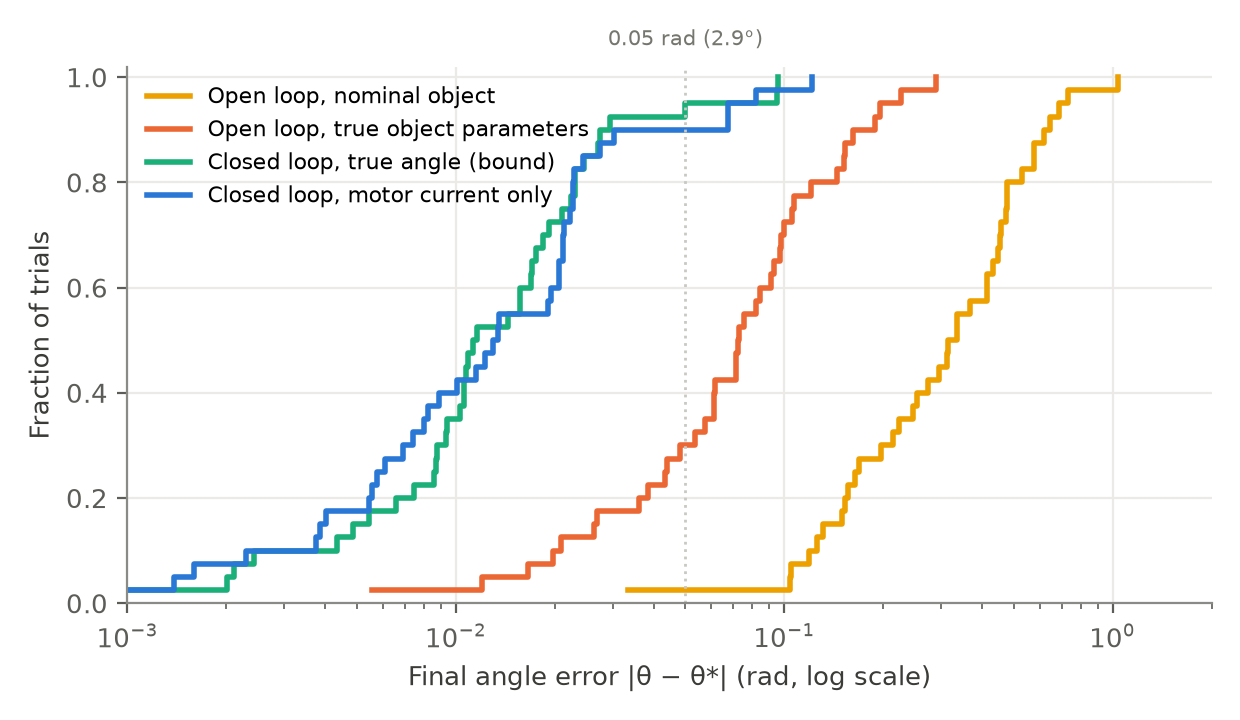
\includegraphics[width=0.66\linewidth]{fig_closed_loop.png}
\caption{Exp C: cumulative distribution of final angle error for the four methods (\Cn{} objects each).}
\label{fig:expC}
\end{figure}

Two qualifications matter. Scored against the object's geometric angle, the closed-loop advantage over the informed open loop narrows to \CCcRod{} versus \COoRod{}\,rad, because the controller targets the COM direction it can observe. The controller is also slow: it used \CCcProbes{} probes on average (at most \CCcProbesMax{}) and \CCcTsim{} simulated minutes per pivot, most of it searching downward for the force at which the object first moves.

\paragraph{A negative result: wrist dither during release.} Our first controller dithered the wrist continuously while the grip was released and tracked $\hat\theta(t)$ with a rolling least-squares window, clamping when the estimate reached the target. It overshot even when fed the true angle. With the grip at the edge of slipping, every half-cycle that raised the gravity torque nudged the object further down, so the dither ratcheted the object past the target. The stepped controller of Section~\ref{sec:controller} keeps the wrist still whenever the grip is low.

\section{Discussion and Limitations}
\paragraph{What torque observes.} Wrist torque measures the direction of the COM about the wrist axis. For slender objects grasped on their centreline this approximates the geometric angle, but in-grasp translation produced a \Agap{}\,rad RMS gap in our simulations. Tasks that need the geometric angle would require a second cue, for instance finger-joint positions or a model of the object's shape.

\paragraph{Simulation only.} All results come from MuJoCo with a soft-finger contact model. The torsional coefficient, the absence of a static--kinetic friction difference, the soft-contact lag and the slip behaviour all affect the numbers. The motor model is idealized: pure Coulomb plus viscous friction with no position-dependent gear ripple, no Stribeck effect, no temperature drift and a linear current--torque map. The grip force is commanded perfectly; on hardware it would itself be set through a current loop. Hardware validation on a low-cost servo gripper is the necessary next step.

\paragraph{Speed.} About \CCcProbes{} ten-second probes per pivot is too slow for most applications. Most probes are spent finding the pivot threshold. Faster sweeps need a two-frequency probe that makes inertia identifiable, and a better prior on $\mu_t$ would shorten the search.

\paragraph{Scope.} One object shape, one grasp geometry and planar pivoting about the grasp axis were studied, with the downhill probe assuming objects that hang no further than vertical.

\section{Conclusion}
The current of a wrist actuator is enough to measure, and to control, the angle of an object pivoting under gravity, in simulation and within the limits above. A slow, downhill wrist sweep with a four-term least-squares fit removes the need to know the object or calibrate the motor, and it tolerates gearbox friction larger than the gravity signal. A converter whose step is no larger than about twice the current noise makes a simple linearized error budget accurate. The approach targets inexpensive grippers that have no tactile sensing, and the next test is whether these results hold on such hardware.

\paragraph{Reproducibility.} The simulation model, motor and sensing-chain model, estimator, controller, raw results and figure scripts accompany this preprint. Every number in this paper is generated from the result files by a script rather than typed by hand.

\paragraph{Use of AI tools.} An AI assistant (Claude, Anthropic) was used to write and debug simulation and analysis code and to draft and edit the text. The author directed the study, reviewed the code and results, and is responsible for the content.

\begin{thebibliography}{99}\small
\bibitem{holladay2015} A.~Holladay, R.~Paolini, and M.~T.~Mason, ``A general framework for open-loop pivoting,'' in \emph{Proc.\ IEEE Int.\ Conf.\ Robotics and Automation (ICRA)}, 2015, pp.~3675--3681.
\bibitem{vina2016} F.~E.~Vi\~na~B., Y.~Karayiannidis, C.~Smith, and D.~Kragic, ``Adaptive control for pivoting with visual and tactile feedback,'' in \emph{Proc.\ IEEE Int.\ Conf.\ Robotics and Automation (ICRA)}, 2016, pp.~399--406.
\bibitem{toskov2023} J.~Toskov, R.~Newbury, M.~Mukadam, D.~Kuli\'c, and A.~Cosgun, ``In-hand gravitational pivoting using tactile sensing,'' in \emph{Proc.\ 6th Conf.\ Robot Learning (CoRL)}, PMLR vol.~205, 2023, pp.~2284--2293.
\bibitem{xydas1999} N.~Xydas and I.~Kao, ``Modeling of contact mechanics and friction limit surfaces for soft fingers in robotics, with experimental results,'' \emph{Int.\ J.\ Robotics Research}, vol.~18, no.~9, pp.~941--950, 1999.
\bibitem{deluca2005} A.~De~Luca and R.~Mattone, ``Sensorless robot collision detection and hybrid force/motion control,'' in \emph{Proc.\ IEEE Int.\ Conf.\ Robotics and Automation (ICRA)}, 2005, pp.~999--1004.
\bibitem{ma2026} C.~Ma, Y.~Yao, Z.~Wei, R.~Li, D.~Szafir, and M.~Ding, ``Current as touch: Proprioceptive contact feedback for compliant dexterous manipulation,'' arXiv:2607.03529, 2026.
\bibitem{shuto2026} Y.~Shuto and D.~V.~Vargas, ``Sensorless damage-safe grasping,'' arXiv:2608.23983, 2026.
\bibitem{zhu2026} Y.~Zhu, J.~Li, Y.~Dong, M.~Suhail, C.~Yang, X.~Luo, H.~Li, B.~Chen, and X.~Cheng, ``CoPRE: Improving sensitivity in proprioceptive contact detection for low-cost robot arms,'' arXiv:2609.27381, 2026.
\bibitem{armstrong1994} B.~Armstrong-H\'elouvry, P.~Dupont, and C.~Canudas de Wit, ``A survey of models, analysis tools and compensation methods for the control of machines with friction,'' \emph{Automatica}, vol.~30, no.~7, pp.~1083--1138, 1994.
\bibitem{gray1993} R.~M.~Gray and T.~G.~Stockham, ``Dithered quantizers,'' \emph{IEEE Trans.\ Information Theory}, vol.~39, no.~3, pp.~805--812, 1993.
\bibitem{todorov2012} E.~Todorov, T.~Erez, and Y.~Tassa, ``MuJoCo: A physics engine for model-based control,'' in \emph{Proc.\ IEEE/RSJ Int.\ Conf.\ Intelligent Robots and Systems (IROS)}, 2012, pp.~5026--5033.
\bibitem{aidoo2026} C.~Aidoo, ``Auditing a slip-induced reorientation study: An evaluation artifact and a corrected gravity-pivoting testbed,'' CANLABS technical report, v2, October 2026.
\end{thebibliography}
\end{document}
